\documentclass[12pt, twoside]{article}
\usepackage{jmlda}
\newcommand{\hdir}{.}
\usepackage[utf8]{inputenc}
\usepackage[english,russian]{babel}
\usepackage{graphicx}
\newcommand{\real}{\mathbb{R}}
\newcommand{\nat}{\mathbb{N}}
\newcommand{\integ}{\mathbb{Z}}
\usepackage{bm}
\usepackage{multicol}

\begin{document}

\title
    [Анализ свойств ансамбля локально аппроксимирующих моделей] % краткое название; не нужно, если полное название влезает в~колонтитул
    {Анализ свойств ансамбля локально аппроксимирующих моделей}
\author
    [Р.\,И.~Исламов, А.\,В.~Грабовой, В.\,В.~Стрижов] % список авторов (не более трех) для колонтитула; не нужен, если основной список влезает в колонтитул
    {Р.\,И.~Исламов, А.\,В.~Грабовой, В.\,В.~Стрижов} % основной список авторов, выводимый в оглавление
    [Р.\,И.~Исламов$^1$, А.\,В.~Грабовой$^1$, В.\,В.~Стрижов$^{1}$] % список авторов, выводимый в заголовок; не нужен, если он не отличается от основного
\email
    {islamov.ri@phystech.edu; grabovoy.av@phystech.edu;  strijov@ccas.ru}
%\thanks
%    {Работа выполнена при
%     %частичной
%     финансовой поддержке РФФИ, проекты \No\ \No 00-00-00000 и 00-00-00001.}
\organization
    {$^1$Московский физико-технический институт}
\abstract
    {Данная работа посвящена анализу свойств ансамбля локальных моделей. Для задачи регрессии  предлагается использовать многоуровневый подход, согласно которому множество объектов разбивается на несколько подмножеств и каждому подмножеству соответствует одна локальная модель. Рассматривается задача построения универсального аппроксиматора --- мультимодели, которая представлена в виде совокупности локальных моделей. В качестве решающей функции используется выпуклая комбинация локальных моделей.  Коэффициенты выпуклой комбинации --- шлюзовая функция --- функция, значение которой зависит от объекта, для которого производится предсказание. Такой подход позволяет описывать те выборки, которые затруднительно описывать одной моделью. Для анализа свойств проводится вычислительный эксперимент. В качестве данных используются синтетические и реальные выборки. В данной работе реальные данные представлены выборками из boston house prices dataset, servo dataset.  
	
\bigskip
\noindent
\textbf{Ключевые слова}: \emph {локальная модель; линейные модели; ансамбль моделей.}
}

\maketitle
\linenumbers

\section{Введение}
В данной работе исследуется проблема построения мультимодели --- ансамбля локальных моделей. \textit{Локальная модель} --- модель, которая обрабатывает объекты, находящиеся в определенной связной области в пространстве объектов. В качестве агрегирующей функции используется выпуклая комбинация локальных моделей, при этом веса локальных моделей не постоянны, а зависят от положения объекта в пространстве объектов. 

Подход к мультимоделированию предполагает, что вклад каждой локальной модели в ответ зависит от рассматриваемого объекта. Мультимодель использует шлюзовую функцию, которая определяет значимость предсказания каждой локальной модели, входящей в ансамбль.

В данной работе каждая локальная модель является линейной. В качестве функционала качества рассматривается логарифм правдоподобия модели. Предлагается алгоритм нахождения оптимальных параметров ансамбля и локальных моделей. 

Преимуществом данного подхода является его способность описывать те выборки, которые затруднительно описывать одной моделью, и разбивать выборку в соответствии с выбранными моделями.

Алгоритмы тестировались на синтетических и реальных данных. Реальные данные представляли собой boston house prices и servo datasets. Эксперименты показали преимущество использования многоуровневой модели и смеси моделей по сравнению с использованием одной модели.


В прикладных задачах данные порождены в результате использования нескольких источников, либо гипотеза порождения и вовсе не известна. В таких случаях качество предсказания можно повышать увеличивая количество моделей. Если моделей на самом деле меньше, чем предполагается, то веса лишних моделей будут малы и их вклад
будет несущественен. Этим объясняется актуальность использования мультимоделирования.

\subsection{Работы по теме}

С момента своего появления мультимодельный подход стал предметом многих исследований. Были предложены различные типы архитектур локальных моделей, такие как SVM \cite{Collobert2002}, Гауссовский процесс \cite{Tresp01mixturesof}  и нейронные сети \cite{Shazeer2017}. Другие работы была сосредоточены на различных конфигурациях, таких как иерархическая структура \cite{NIPS1991_514}, бесконечное число экспертов \cite{Rasmussen} и последовательное добавление экспертов \cite{Aljundi2016}. \cite{garmash-monz-2016-ensemble} предлагает модель ансамбля локальных моделей для машинного перевода. Стробирующая сеть обучается на предварительно обученной модели NMT ансамбля. 

Ансамбль локальных моделей имеет множество приложений в прикладных задачах. Работы \cite{Yumlu2003}, \cite{Cheung1995}\cite{Weigend2000} посвящены применению смеси экспертов в задачах прогнозирования временных
рядов. В работе \cite{article} предложен метод распознавания рукописных цифр. Метод распознания текстов при помощи ансамбля локальных моделей исследуется в работах \cite{Estabrooks2001}, а для распознавания речи --- в \cite{Mossavat2010}, \cite{Peng1996}. В работе \cite{Sminchisescu2007} исследуется смесь экспертов для задачи распознавания трехмерных движений человека.

\section{Постановка задачи построения ансамбля локальных моделей}
Пусть задано множество объектов $\Omega$. Будем считать, что множество объектов разбивается на $k$ непересекающихся подмножеств $\Omega_k$:
\[\Omega = \bigsqcup_{k=1}^K \Omega_k. \eqno(3.1)\]
Также задано $\Omega', |\Omega'| = N$ --- множество объектов для обучения,  являющееся подмножеством $\Omega$. Предполагается, что в $\Omega'$ представлены объекты из всех подмножеств $\Omega_k$:

\[\Omega' = \bigsqcup_{k=1}^K \Omega_k', \eqno(3.2)\]
где $\Omega_k' \subset \Omega_k$. Пусть задан вектор $\mathbf{y} \in \real^N$ --- вектор правильных ответов. Разбиение множества объектов $\Omega'$ на подмножества индуцирует разбиение вектора $\mathbf{y}$ на подвекторы $\mathbf{y}_k$. 

Для каждого объекта из $\Omega$ задано признаковое описание в соответствии с подмножеством, в котором объект находится. Это отображение $\mathcal{K}_k$ из множества объектов в пространство признаков:
\[\mathcal{K}_k: \Omega_k \rightarrow \real^{n_k}, k \in \overline{1, K}. \eqno(3.3)\]
В качестве общего пространства признаков будем рассматривать $\real^n = \real^{n_1} \times \dotsc \times \real^{n_K}$, полным признаковым описанием объекта является вектор $\mathbf{x} = [\mathbf{x}^1, \mathbf{x}^2, \dotsc, \mathbf{x}^K]$. Введем  выборку данных $\mathcal{D}$:
\[\mathcal{D} = \{(\mathbf{x}_i, y_i)~|~i \in \overline{1, N}\}, \eqno(3.4)\]
где $\mathbf{x}_i \in \real^n$ --- полное признаковое описание объекта из $\Omega'$, а $y_i \in \real$ --- значение целевой переменной, соответствующее этому объекту.
Для каждого подмножества используется своя локальная модель.\\
\begin{Definition}
\label{def:1}
Модель $\mathbf{g}_k$ называется локальной, если она аппроксимирует некоторую пару $(\Omega_k', \mathbf{y}_k)$.
\end{Definition}
В приведенном определении подразумевается, что локальная модель $\mathbf{g}_k$ использует только соответствующее признаковое описание $\mathbf{x}^{k}_i \in \real^{n_k}$ объекта --- подвектор вектора $\mathbf{x}_i$, соответствующий отображению $\mathcal{K}_k$. В данной работе локальный модели объединены в ансамбль локальных моделей.\\
\begin{Definition}
\label{def:2}
Ансамбль локальных моделей --- мультимодель, определяющая правдоподобие веса $\pi_k$ каждой локальной модели $\textbf{f}_k$ на признаковом описании объекта $\textbf{x}$.
\[\mathbf{f} = \sum\limits_{k=1}^K\pi_k\mathbf{g}_k(\mathbf{x}^{k},\mathbf{w}_k),\qquad \pi_k\left(\mathbf{x}, \mathbf{V}\right): \real^{n\times |\mathbf{V}|} \rightarrow [0,1], \qquad \sum\limits_{k=1}^K\pi_k\left(\mathbf{x}, \mathbf{V}\right) = 1, \eqno(3.5)\]
$\mathbf{f}$ --- мультимодель, $\mathbf{g}_k$ --- локальная модель, $\pi_k$ --- шлюзовая функция, $\mathbf{V}$--- параметры шлюзовой функции. 
\end{Definition}



В данной работе в качестве локальной модели $\mathbf{g}_k$ и шлюзовой функции $\bm{\pi}$ рассматриваются следующие функции:

\[\mathbf{g}_k(\mathbf{x}^{k}, \mathbf{w}_k) = \mathbf{w}_k^{\mathsf{T}}\mathbf{x}^{k}, \qquad \bm{\pi}\left(\mathbf{x}, \mathbf{V}\right) = \text{softmax}\left(\mathbf{V}_1^{\mathsf{T}}\sigma\left(\mathbf{V}_2^{\mathsf{T}}\mathbf{x}\right)\right), \eqno(3.6)\]
где $\mathbf{V} = \{\mathbf{V}_1, \mathbf{V}_2\}$ --- параметры шлюзовой функции, $\sigma(x)$ --- сигмоидная функция. Введем понятие расстояние между двумя объектами.\\
\begin{Definition}
\label{def:3}
Расстоянием между двумя объектами $\omega_1$ и $\omega_2$ из $\Omega$ называется число, равное расстоянию между векторами признаковых описаний этих объектов, и вычисляемое по формуле

\[\rho(\omega_1, \omega_2) = \left|\left|\mathcal{K}_1(\omega_1) - \mathcal{K}_1(\omega_2), \mathcal{K}_2(\omega_1) -  \mathcal{K}_2(\omega_2), \dotsc, \mathcal{K}_k(\omega_1) -  \mathcal{K}_k(\omega_2)\right|\right|_2. \eqno(3.7) \]
\end{Definition} 
Будем считать, что каждый объект имеет векторное описание $\mathbf{x}$, взятый из некоторого вероятностного распределения. Пусть этому распределению соответствует вероятностная мера $\mathsf{F}(x)$ в пространстве признаковых описаний объектов. Тогда пространство локальных моделей является гильбертовым пространством, в котором введено скалярное произведение.\\
\begin{Definition}
\label{def:2}
Скалярным произведением между двумя локальными моделями $\mathbf{g}_i$ и $\mathbf{g}_j$ называется число, вычисляемое по формуле
\[ \left<\mathbf{g}_i, \mathbf{g}_j\right> = \mathbb{E}\left[\mathbf{g}_i(\mathbf{x}^i, \mathbf{w}_i),\mathbf{g}_j(\mathbf{x}^j, \mathbf{w}_j) \right], \eqno(3.8)\]
где $\mathbb{E}\left[\xi, \eta\right] = \int\limits_{\real^n}\xi(\mathbf{x})\eta(\mathbf{x})\mathsf{dF}(\mathbf{x})$ --- математическое ожидание произведения случайных величин.
\end{Definition}


Для нахождения оптимальных параметров мультимодели используется функция ошибки следующего вида:
\[\mathcal{L}\left(\textbf{V}, \textbf{W}\right) = \sum\limits_{(\textbf{x}, y) \in \mathcal{D}} \sum\limits_{k=1}^K\pi_k\left(\textbf{x}, \textbf{V}\right)\left(y - \textbf{w}_k^{\mathsf{T}}\textbf{x}^k\right)^2 + R\left(\mathbf{V}, \mathbf{W}\right), \eqno(3.9)\] 
где $\mathbf{W} = [\mathbf{w}_1, \mathbf{w}_2, \dotsc, \mathbf{w}_k]$ --- параметры локальных моделей, $R\left(\mathbf{V}, \mathbf{W}\right)$ --- регуляризация параметров.

\section{Вычислительный эксперимент}

\subsection{Постановка проблемы}

В данном эксперименте изучается проблема, когда выборка имеет не одну порождающую модель, а несколько. В качестве данных используются синтетическая выборка. Создается две подвыборки объектов, описываемых линейной моделью с нормальным шумом. В каждом подвыборке объекты имеют один признак. Будем обозначать признак объектов из первого подмножества как $x_1$, а признак объектов из второго подмножества как $x_2$. Эти две подвыборки сливаются в одну общую выборку. 

В первом эксперименте для объектов из одного подмножества признаки, соответствующие другому подмножеству, берутся нулевыми. На общей выборке обучается линейная модель. Так как признаки объектов, соответствующие другой подвыборке, взяты нулевыми, то это никак не мешает модели обучаться на общих данных. Точность предсказания при таком построении модели высока.

Во втором эксперименте признаки объектов, не соответствующие подмножеству, берутся из нормального распределения $\mathcal{N}(0,1)$, то есть признаки становятся зашумленными, при этом все также используется одна общая модель. Такое построение общей выборки усложняет обучение линейной модели, так как разделение объектов на принадлежность подмножеству становится труднее. Следствием этого является снижение точности предсказания.


\begin{figure}[h]
\begin{center}
\begin{minipage}[h]{0.49\linewidth}
\begin{center}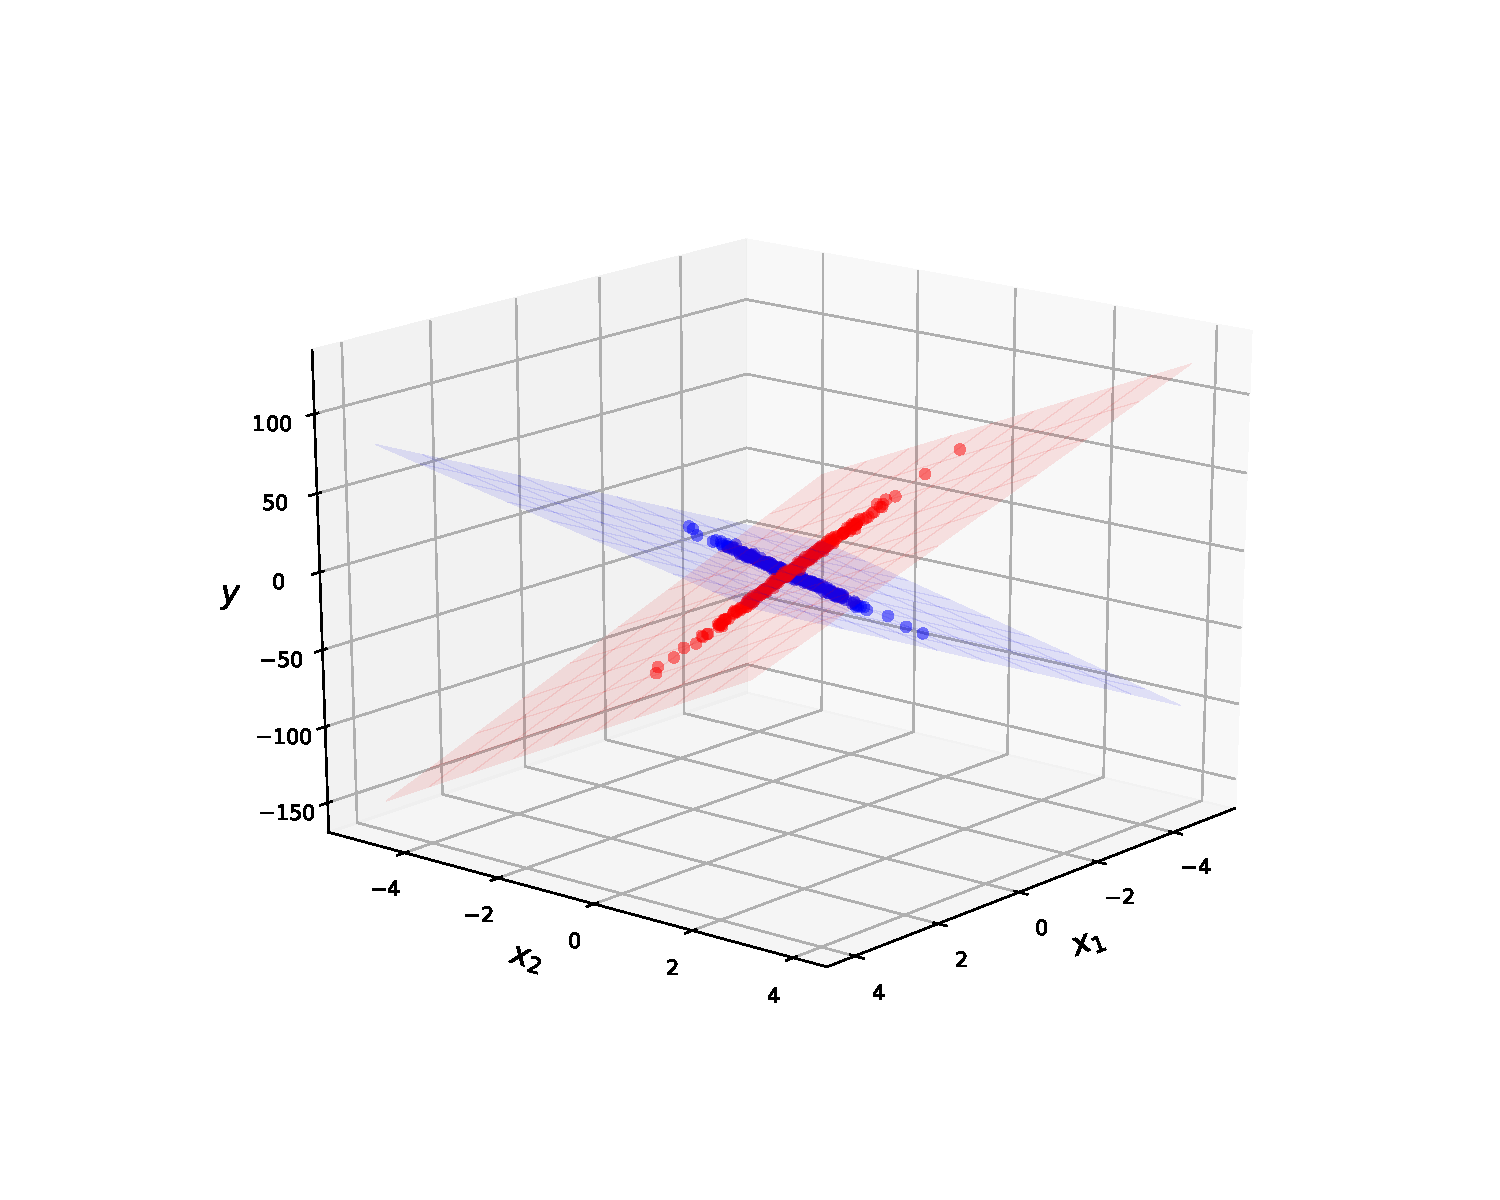
\includegraphics[width=1.2\linewidth]{experiment1-zeros.pdf}  а) \end{center}
\end{minipage}
\hfill
\begin{minipage}[h]{0.49\linewidth}
\begin{center}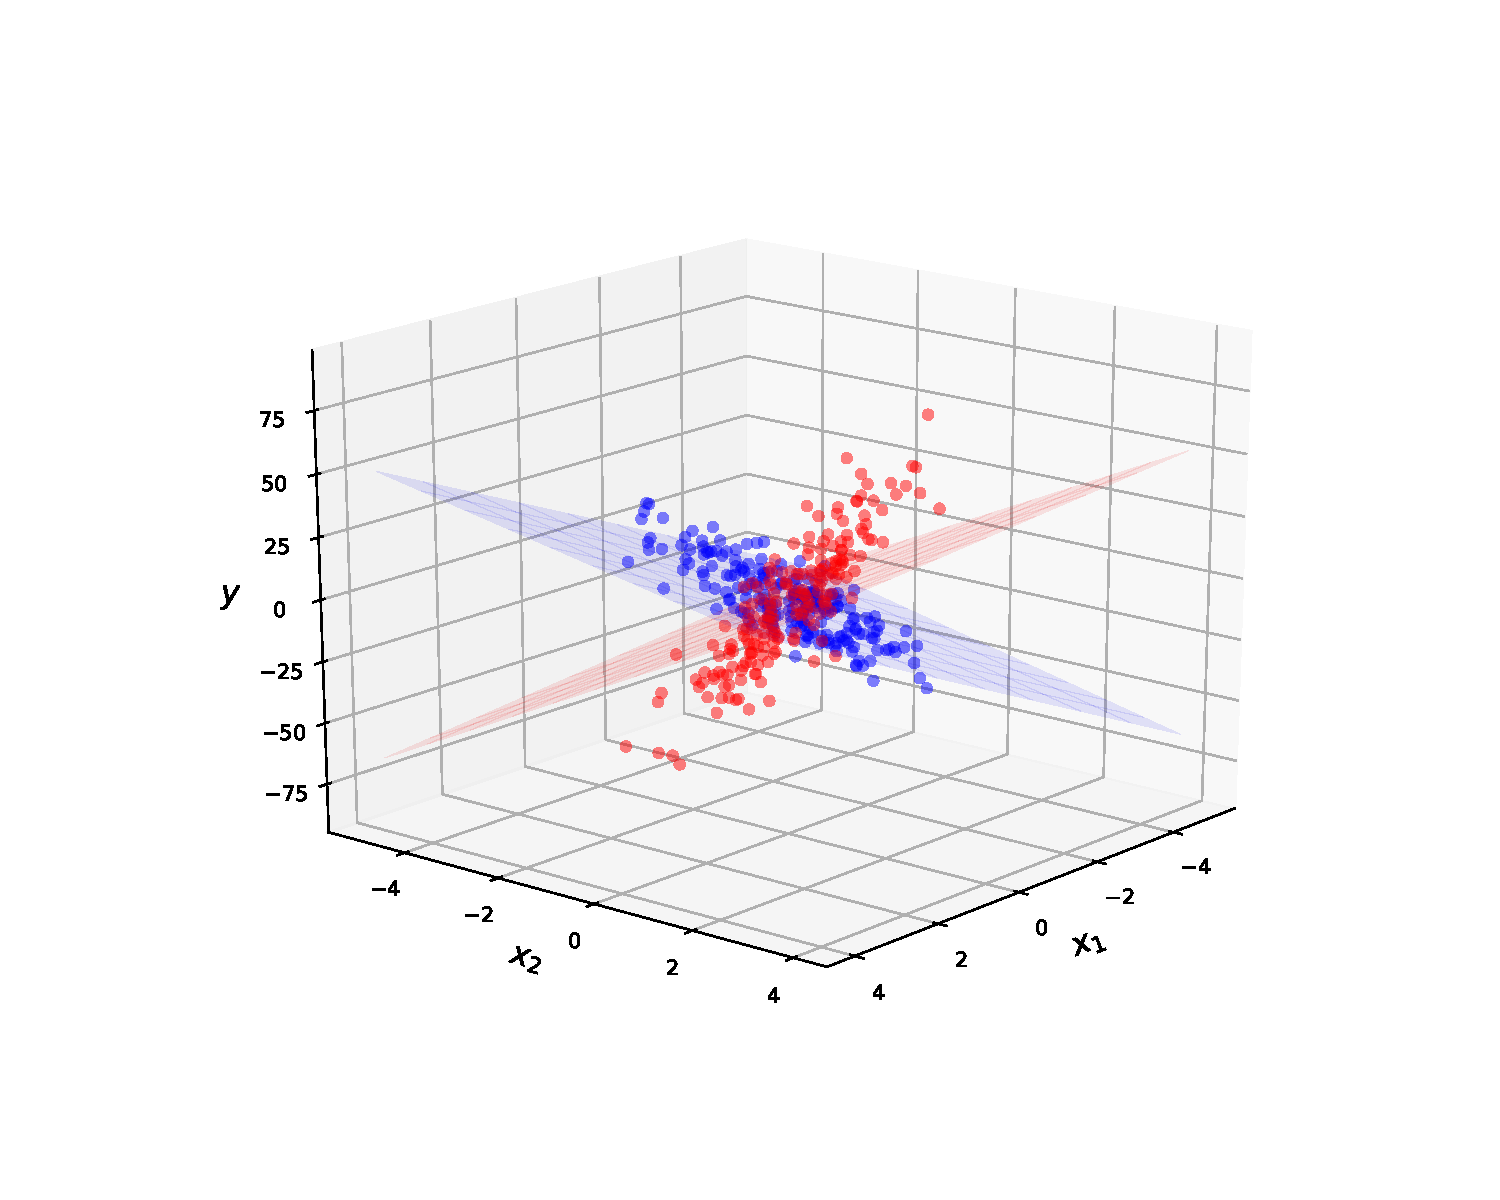
\includegraphics[width=1.2\linewidth]{experiment1-random.pdf}  б) \end{center}
\end{minipage}
\caption{а) Признаки, соответствующие другому подмножеству, заполнялись нулями, б) признаки, соответствующие другому подмножеству, заполнялись случайными числами. Точки соответствуют правильным ответам, плоскости задают предсказание линейной модели для каждого из подмножеств.}
\label{ris:image1}
\end{center}
\end{figure}


Таким образом, при построение модели для обучения нужно учитывать гипотезу порождения данных. Нередко оказывается, что данные порождены не одним источником, а несколькими. В этом случае лучше использовать мультимодель --- совокупность локальных моделей, где каждая локальная модель обрабатывает свою область признакового пространства (в одной области объекты имеют схожие признаки, объекты из разных областей имеют разные признаковые описания).

\subsection{Базовый алгоритм. Построение ансамбля локальных моделей}

В данном эксперименте используется мультимодель с двумя линейными локальными моделями. Обучение этого ансамбля локальных моделей происходит в два этапа: на первом этапе оптимизируются параметры локальных моделей, на втором --- параметры шлюзовой функции. Используется те же два подхода построения общей выборки, как и в предыдущем пункте. 

В первом эксперименте для объектов из одного подмножества признаки, соответствующие другому подмножеству, берутся нулевыми. При обучении мультимодели на такой выборке параметры локальных моделей становятся близкими друг к другу. Это объясняется тем, что для аппроксимации данной выборки достаточно одной локальной модели.

Во втором эксперименте признаки объектов, не соответствующие подмножеству, берутся из нормального распределения $\mathcal{N}(0,1)$. В данном эксперименте мультимодель обучается так, что каждая локальная модель аппроксимирует одно из подмножеств. Параметры локальных моделей получаются близкими к нужным: один из коэффициентов близок к коэффициенту, при помощи которого порождалось подмножество, а второй --- к нулю. В данном случае двух локальных моделей достаточно для аппроксимации общей выборки. 

\begin{figure}[h]
\begin{center}
\begin{minipage}[h]{0.49\linewidth}
\begin{center}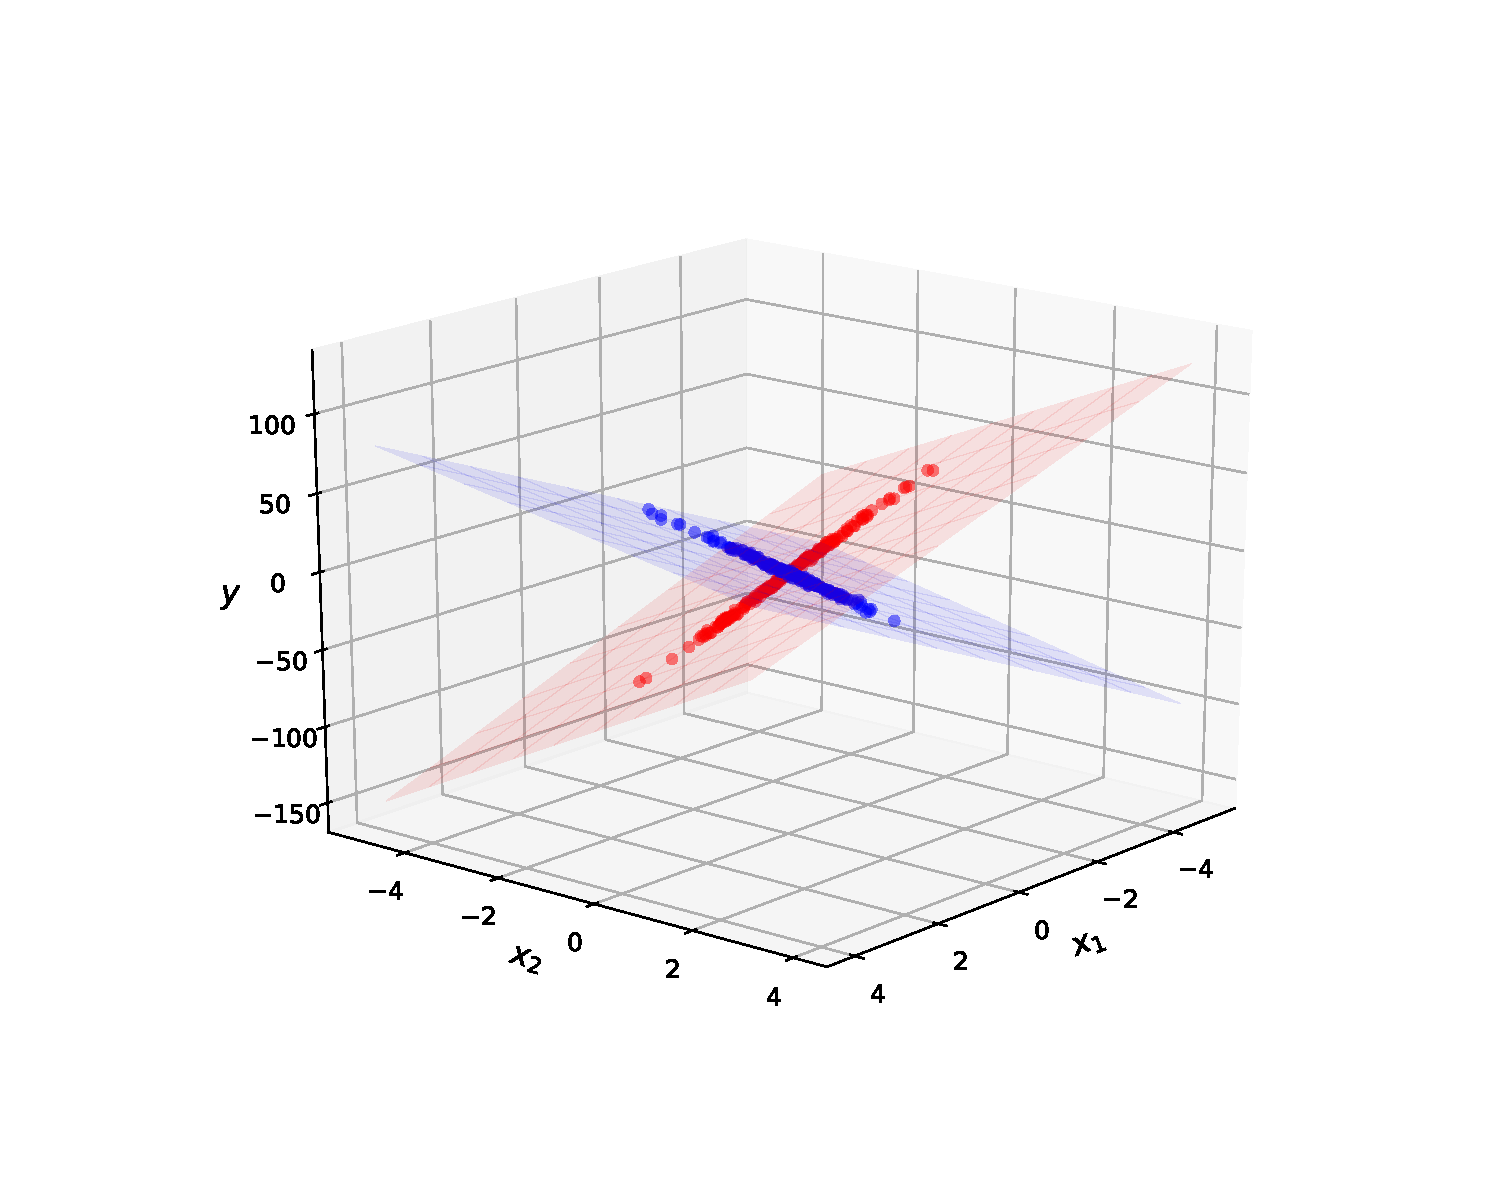
\includegraphics[width=1.2\linewidth]{experiment2-zeros.pdf}  а) \end{center}
\end{minipage}
\hfill
\begin{minipage}[h]{0.49\linewidth}
\begin{center}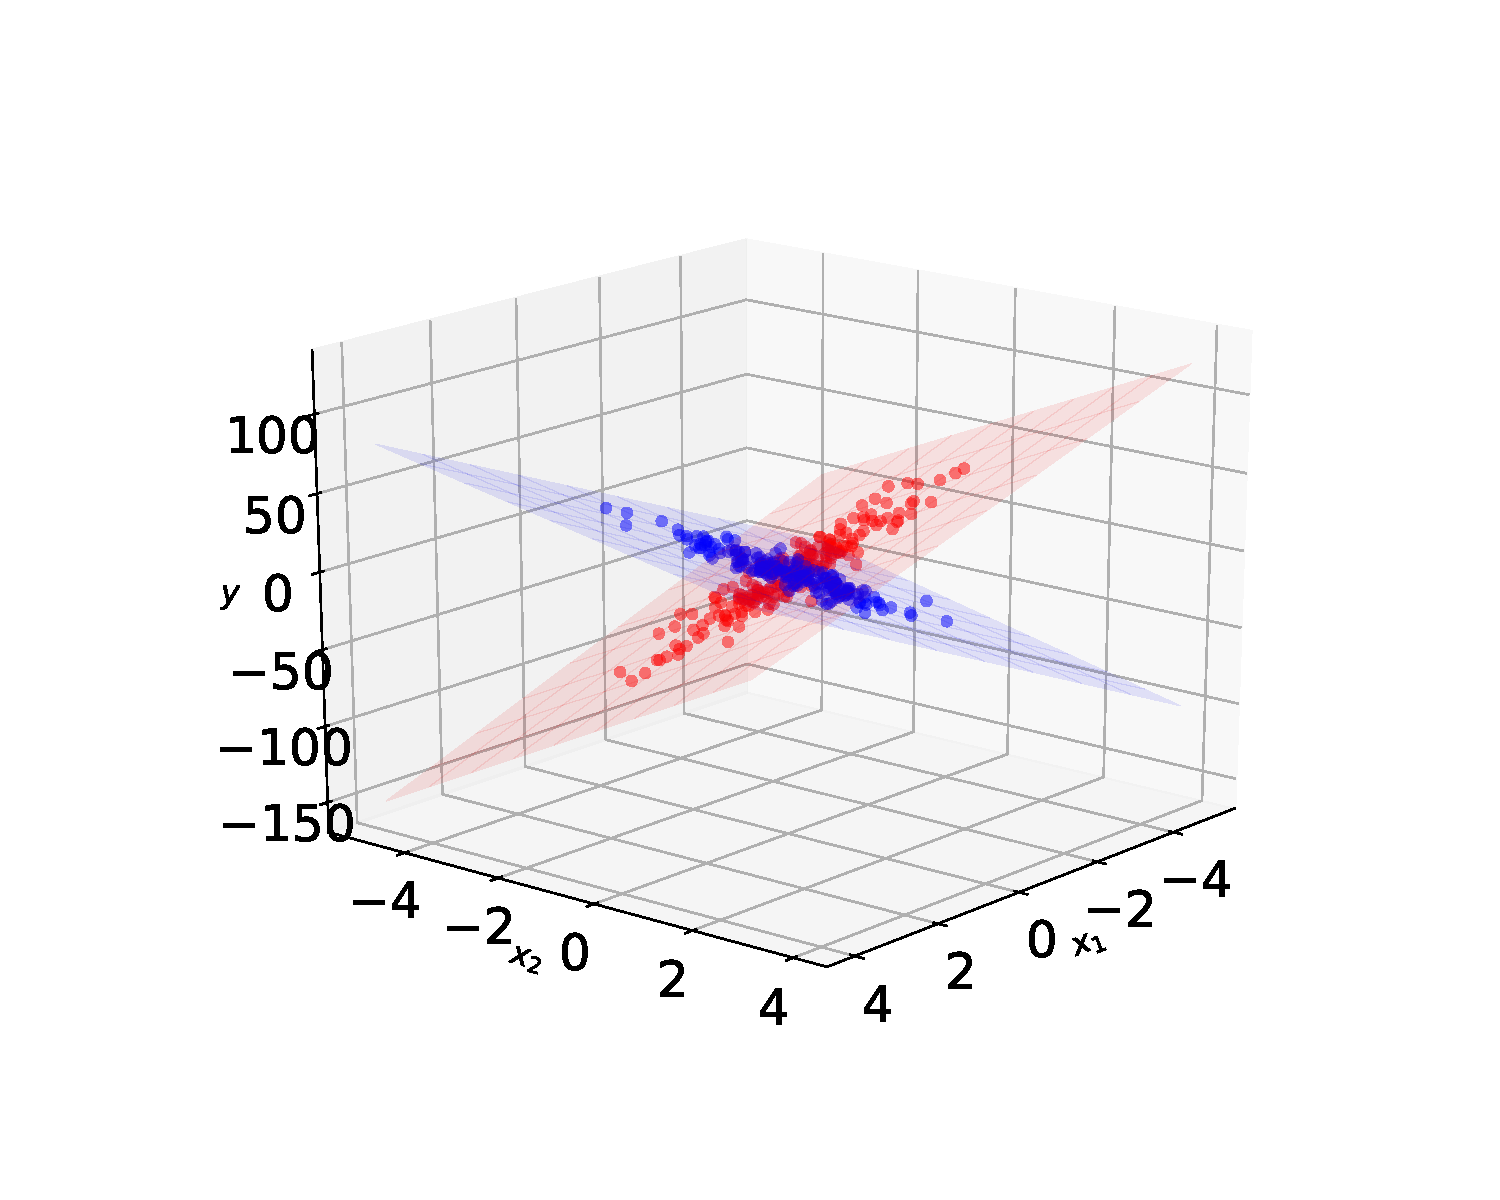
\includegraphics[width=1.2\linewidth]{experiment2-random.pdf}  б) \end{center}
\end{minipage}
\caption{а) Признаки, соответствующие другому подмножеству, заполнялись нулями, б) признаки, соответствующие другому подмножеству, заполнялись случайными числами. Точки соответствуют правильным ответам, плоскости задают предсказание мультимодели для каждого из подмножеств.}
\label{ris:image1}
\end{center}
\end{figure}



\bibliographystyle{unsrt}
\bibliography{Islamov}

\end{document}
